\documentclass[conference]{IEEEtran}
\IEEEoverridecommandlockouts
% The preceding line is only needed to identify funding in the first footnote. If that is unneeded, please comment it out.
%Template version as of 6/27/2024

\usepackage{cite}
\usepackage{amsmath,amssymb,amsfonts}
\usepackage{algorithmic}
\usepackage{graphicx}
\usepackage{textcomp}
\usepackage{xcolor}
\usepackage{longtable}
\usepackage{booktabs}
\usepackage{tabularx}
\usepackage{array}
\usepackage{graphicx}
\usepackage{hyperref}
\usepackage{listings}
% \usepackage{fontspec}      % 支持字体选择,XeLaTeX/LuaLaTeX 必需
% \usepackage{xeCJK}         % 支持中文,自动处理中文断行和字体
% \setmainfont{Times New Roman}  % 英文字体
% \setCJKmainfont{Noto Serif CJK SC} % 中文字体
\def\BibTeX{{\rm B\kern-.05em{\sc i\kern-.025em b}\kern-.08em
    T\kern-.1667em\lower.7ex\hbox{E}\kern-.125emX}}

\begin{document}

\section{Contextual Structure Expression: A Unified Modeling Framework
for Semantic Contextual
Markup}\label{contextual-structure-expression-a-unified-modeling-framework-for-semantic-contextual-markup}

Liwei Zhao

Independent Researcher

April 21, 2025

\subsection{Abstract}\label{abstract}

With the development of large language models (LLMs), knowledge has
gradually replaced information as the core object of processing, and the
focus of structured expression is quietly shifting.

Traditional structured expressions, represented by JSON, YAML, RDF,
etc., are limited by static structures and deterministic assumptions,
making them difficult to meet the needs of a semantics-driven era. In
intelligent systems, the actual semantics often depend on changes in
contextual background. The preset schema approach becomes extremely
rigid when dealing with dynamically changing contexts. Moreover, because
LLMs are better at processing natural language, using JSON, YAML, or RDF
to exchange semantics leads to frequent conversions between these
formats and natural language. During the linearization process, a
certain degree of semantic loss occurs, ultimately leading to contextual
inconsistencies and various issues in multimodal collaboration, dynamic
context binding, and explainability.

This is fundamentally a generational disparity issue, as these formats
were created for information exchange rather than for expressing
semantic relationships.

To address this, this paper proposes a minimalist expression paradigm
for semantic modeling --- Contextual Structure Expression (CSE), and
based on this paradigm, designs Context Mark Language (CML), which
prioritizes semantic structure expression and can be embedded within
natural language. It demonstrates significant advantages in the marking,
transmission, storage, sharing, and computation of context, showing vast
potential in the standardization and generalization of semantic
relationship expression.

\subsection{1. Introduction}\label{1-introduction}

In recent years, large language models (LLMs) have achieved
groundbreaking progress in natural language understanding and
generation.

\subsubsection{1.1. Background}\label{11-background}

With the widespread adoption of generative AI and large language models
(LLMs), natural language processing is entering a new phase---one that
relies more heavily on semantic structures and contextual reasoning.

However, current research and applications of LLMs are still primarily
focused on knowledge lifecycle management, including processes such as
knowledge acquisition, representation, reasoning, and generation. In
existing systems, contextual semantics are typically treated as
unstructured and ephemeral inputs. There is still a lack of systematic
modeling paradigms and intermediary protocols, making this a key
bottleneck in the advancement of LLM-driven intelligence.

\subsubsection{1.2. The Paradigm Problem}\label{12-the-paradigm-problem}

The paradigms for semantic representation and semantic storage are among
the most pressing challenges facing the industry today.

On one hand, most mainstream AI models still rely heavily on offline
training to acquire knowledge. This approach embeds knowledge directly
into model parameters, resulting in poor consistency and making it
difficult to support high-frequency updates to knowledge versions. Once
distilled into the model, knowledge becomes internal weight
parameters---effectively ``frozen semantics.'' These cannot be modified,
recombined, or interpreted, making it extremely difficult for external
systems to manage knowledge flexibly at the contextual level. This
structural limitation leads to a high cost for knowledge iteration,
which is particularly detrimental for regulatory documents and
time-sensitive professional knowledge, causing slow updates {[}1{]} and
significant lag.

Although the widely adopted RAG (Retrieval-Augmented Generation)
framework enables dynamic knowledge injection to some extent {[}2{]}, in
essence, it only shifts the problem of ``freezing'' from inside the
model to an external retrieval database. The form changes---from model
parameters to vector fragments---but the fundamental issue remains
unresolved.

On the other hand, existing semantic representation formats such as RDF
and JSON-LD {[}3{]} do offer structural precision, but they fall short
in terms of lightweight flexibility. Their annotation formats are quite
distant from the natural language form that LLMs are designed to work
with, which creates significant limitations in embedding, transmission,
storage, multimodal sharing, compositional operations, and linear
transformations.

Moreover, these formats generally emphasize static structures and
explicitly annotated numerical weights. Static structures impose
semantic constraints through predefined schemas, but due to differences
in expression standards across modalities and models, they inherently
lack general-purpose, cross-modal, and cross-model alignment
capabilities {[}4{]}. Meanwhile, explicit numerical weights struggle to
accurately represent the implicit relationships, semantic ambiguity, and
dynamic intent present in natural language dialogues and
tasks---it\textquotesingle s a kind of "false precision".

A more promising direction is to achieve a decoupling of semantic
structure representation and weight quantification at the architectural
level. This would allow contextual semantic structures to be managed
independently, and even upstream at the knowledge source---retaining the
original context during the storage phase, and combining it dynamically
with the runtime context (or different context-aware algorithms) for
on-the-fly reasoning and weight computation.

In such a framework, semantic structures can evolve independently
{[}5{]}, without being constrained by any specific model or modality's
weighting strategy---thus enabling a pluggable, evolvable, reusable, and
interpretable system for semantic modeling.

\subsubsection{1.3. A New Paradigm for Semantic Expression:
CSE}\label{13-a-new-paradigm-for-semantic-expression-cse}

To meet the emerging demands of semantic structure modeling in the era
of LLMs, CML (Context Mark Language) introduces a novel contextual
semantic expression model called Contextual Structure Expression
paradigm(CSE).

CSE adopts a linear composition format of ``semantic tokens + relational
delimiters'', representing multi-dimensional semantic information and
its weight structure using a natural language-compatible string. This
approach---based on a single string, encoding only semantic structure,
and supporting compositional operations---offers clear advantages over
traditional static, structured annotation languages:

\begin{itemize}
\item
  Lightweight for storage and embedding, enabling seamless integration
  with a wide variety of frameworks and formats.
\end{itemize}

\begin{itemize}
\item
  Model-agnostic and modality-neutral, independent of any specific
  quantization strategy, making it a universal semantic intermediary
  format for sharing context across multi-agent, multi-model, and
  multi-modal systems.
\item
  Human-readable, embodying a ``what-you-see-is-the-semantic'' property
  that naturally supports interpretability, semantic restoration and
  reconstruction, traceability, and human-AI collaboration.
\item
  Ability to freely combine operations, empowering dynamic reasoning
  chains and task decomposition with flexible recombination and semantic
  orchestration.
\end{itemize}

These advantages make it possible for CSE to become the "Context
Interlingua" of the AI era and play an infrastructural role in future
evolution.

\subsubsection{1.4. Structure of This
Paper}\label{14-structure-of-this-paper}

The main content of this paper is organized as follows:

\begin{itemize}
\item
  An exposition on semantic loss and generational gaps in statically
  structured languages;
\item
  An analysis of semantic freezing caused by the coupling of logical
  architectures;
\item
  the Contextual Structure Expression (CSE) design;
\item
  the Context Mark Language (CML) specification;
\item
  A comparative analysis between CML and mainstream expression formats;
\item
  Conclusion and future prospects
\item
  References involved or recommended in this paper.
\end{itemize}

\subsection{2. Related Solutions and
Limitations}\label{2-related-solutions-and-limitations}

Currently, within the LLM ecosystem, statically structured languages
(such as JSON, YAML, RDF) continue to play important roles in several
key stages:

\begin{itemize}
\item
  Data Ingestion {[}6{]}: Used to represent structured knowledge such as
  user profiles, knowledge graphs, and API configurations, embedded into
  model input through prompt templates;
\item
  Training Data Construction {[}7{]}: Serve as a mechanism for
  generating supervised corpora and aligning structured semantics (e.g.,
  semantic triples);
\item
  Inference and Task Execution {[}8{]}: Structured data is re-serialized
  into natural language prompts to support complex tasks such as RAG and
  multimodal question answering.
\end{itemize}

However, such value is primarily of engineering significance, rather
than semantics-centered value.

\subsubsection{2.1. Expression Paradigm
Issues}\label{21-expression-paradigm-issues}

Challenges at the Semantic Expression Layer.

While the current LLM industry primarily focuses on the knowledge
lifecycle---that is, how to ingest, train, infer, and update---static
structured languages such as JSON, YAML, and RDF have indeed proven
sufficient for engineering systems. However, when the focus shifts to
the semantic lifecycle---including how to annotate, transmit, store,
manage, compute dynamically, perform semantic reasoning, and align
across modalities {[}9{]}---these engineering-driven solutions reveal
significant limitations.

\begin{table*}[htbp]
\centering
\begin{tabularx}{\textwidth}{l>{\raggedright\arraybackslash}X>{\raggedright\arraybackslash}X}
\toprule
Dimension & Characteristics & Impact \\
\midrule
Static Structure & 
Relies on predefined schemas and nested hierarchies, with semantic binding constrained by fixed field names and structural levels. & 
Fails to provide cross-platform consistency and struggles to support LLM dynamic task modeling. \\

Semantic Loss & 
Lacks mechanisms for expressing temporal order, intention hierarchy, or logical progression---It is not conducive to LLM alignment, especially in complex scenes. & 
The process of linearizing structured semantics into prompts and embedding them into rigid formats is essentially a ``downgrade-style'' bridge, inevitably causing semantic compression and contextual distortion. \\
\bottomrule
\end{tabularx}
\label{tab:your_label}
\end{table*}


The original intent of statically structured languages is information
exchange and storage, not complex semantic modeling or dynamic
reasoning.

Although LLMs can \textquotesingle understand\textquotesingle{} JSON and
YAML, there is a significant morphological gap between these formats and
natural language. The transformation process of natural language $\leftrightarrow$
structured formats $\leftrightarrow$ natural language inevitably incurs semantic loss,
making such approaches inadequate---and certainly not optimal---as a
mode of semantic representation.

Fundamentally, this reflects the problem brought about by
intergenerational differences in paradigms: what the industry truly
needs is a semantic interface, not merely a data interface.

\subsubsection{2.2. Semantic Freezing
Problem}\label{22-semantic-freezing-problem}

Challenges at the Semantic Storage Layer.

As mentioned in the introduction, LLMs heavily rely on offline training
paradigms, leading to semantics being frozen within model parameters in
the form of weights. This makes it difficult for external systems to
manage semantic context flexibly and cost-effectively. As a result,
knowledge updates essentially equate to retraining the model---a costly
endeavor that ultimately manifests as slow knowledge updates on the user
side.

On one hand, due to the tight coupling between weight parameters and
model structures (e.g., number of layers, attention mechanisms), the
original semantic structure is irreversibly compressed during training
and frozen into the model's architecture. This makes semantics hard to
reuse or port across platforms.

On the other hand, the quality of these ``frozen'' semantic
representations depends heavily on the algorithms, training data, and
the quality of the original knowledge during the training stage.
However, because the original semantic structure is lost, it is
impossible at runtime to leverage new algorithms, updated corpora, or
refined semantic annotations for low-cost correction. Even if a
knowledge source provides higher-quality semantic labels, the model is
unable to dynamically integrate them.

While RAG seemingly provides LLMs with dynamic access capability, it
does not fundamentally solve the update timeliness required by users
(e.g., second-level and minute-level updates).

This is not merely an engineering challenge---it stems from structural
limitations in the Transformer architecture\textquotesingle s approach
to semantic representation and storage. A more promising direction lies
in decoupling semantic structure expression from weight quantization at
the architectural level.

\begin{itemize}
\item
  Treat the semantic structure as a universal intermediate
  representation, independent of model parameters and externalized from
  the model itself.
\item
  This intermediate representation is conceptually similar to the role
  of ONNX in serving as a universal exchange format for neural networks
  {[}10{]}, but instead of computational graphs, it focuses on
  representing semantic relationships, intended for explicit storage of
  original contextual semantics.
\end{itemize}

Once decoupled:

\begin{itemize}
\item
  Semantics can be extracted from the model architecture and treated as
  platform-independent formatted data, enabling uniform parsing and
  processing across different model types and modalities.
\item
  Semantics can evolve independently of the original knowledge text.
  External systems will be able to directly read, edit, or extend
  them---enabling the concept of Semantic-as-a-Service.
\item
  Model weights would no longer be the sole carrier of knowledge. If
  both training and inference are centered around general semantic
  structures, it opens the door to a new class of LLM architectures that
  only interpret semantic expressions rather than bear the full burden
  of knowledge retention. From a knowledge perspective, this
  significantly lowers the cost of updates and increases reusability and
  flexibility. From an AI engineering standpoint, it also brings
  stronger controllability, explainability {[}11{]}, and algorithmic
  adaptability.
\end{itemize}

\subsubsection{2.3. Direction}\label{23-direction}

To conclude, the AI era may call for a native semantic interlingua
(Context Interlingua)---a foundational layer of infrastructure for the
future of intelligent systems. This is a role that traditional static
structural languages such as JSON, YAML, and RDF were never designed to
fulfill, nor are they capable of evolving into.

In the following sections, we introduce the proposed paradigm of
Contextual Structure Expression (CSE) for dynamic semantic modeling,
along with its concrete implementation: the Context Mark Language (CML).
We then explore the broader prospects of these innovations in driving
the standardization and generalization of semantic expression in the age
of LLMs.

\subsection{3. CSE Expression Paradigm
Design}\label{3-cse-expression-paradigm-design}

Contextual Structure Expression (CSE) is a paradigm centered on
contextual dimensions, presenting a fundamentally different approach in
terms of semantic architecture, expression form, and structural
representation.

\subsubsection{3.1. Example}\label{31-example}

Let's Start with Examples

\begin{table*}[htbp]
\centering
\begin{tabular}{ll}
\toprule
CSE Expression & Semantic Interpretation \\
\midrule
\texttt{message}:\texttt{urgent}+\texttt{alert}@\texttt{user123} &
A message with the nature of ``urgent'' and ``alert,'' targeted at user123 \\
\texttt{task}.\texttt{create}:\texttt{document}@\texttt{project}.\texttt{alpha} &
A task to create a document within project alpha \\
\texttt{question}.\texttt{ai}.\texttt{model}+\texttt{language} &
A compound question about AI, models, and language \\
\texttt{error}.\texttt{timeout}.\texttt{network}@\texttt{device} &
A network-related error of type ``timeout'' occurring on a device \\
\bottomrule
\end{tabular}
% \caption{Your caption here (optional)}
% \label{tab:cse_expression}
\end{table*}


The above are representative examples of CML (Context Mark Language)
plaintext semantic formats. They are highly human-readable, close to
natural language, and friendly to semantic parsing, structural
reconstruction, reasoning path tracing, indexing, and interpretability.

As seen from the CML examples, one of the core design goals of CSE is to
enable concise, flexible, and intuitive expression of semantically rich
contextual structures.

\subsubsection{3.2. Linear Structure}\label{32-linear-structure}

CSE adopts a single-string linear text format that is compatible with
natural language, serving as the carrier for semantic structural
expression. The primary motivation behind this choice is to avoid
semantic loss caused by repeated transformations between natural
language $\leftrightarrow$ structured format $\leftrightarrow$ natural language.

\subsubsection{3.3. Primitive
Architecture}\label{33-primitive-architecture}

The semantic string in the CSE paradigm is composed of a sequence of
semantic primitives, which include two types: semantic tokens and
relation separators.

\begin{itemize}
\item
  Semantic Tokens are the fundamental units for describing contextual
  semantics. They can be any word or short phrase in textual form. While
  conceptually analogous to "tokens" in the LLM domain, they are not
  lexical in nature but represent abstract semantic dimensions that
  carry natural meaning.
\item
  Relation Separators are symbolic delimiters used to represent semantic
  relationships between tokens, implicitly indicating priority weight in
  their connections. These separators---such as @, ., :, +, and
  space---are statically defined, with explicit hierarchical semantics
  and structural roles.
\end{itemize}

\subsubsection{3.4. Semantic Expression
Rules}\label{34-semantic-expression-rules}

We use \texttt{\textless{}semantic\_token\textgreater{}}to denote a
semantic token, and \texttt{\textless{}separator\textgreater{}} to
denote a relation separator. The expression rules are defined as
follows:

\begin{itemize}
\item
  \begin{sloppypar}
  Each semantic token
  (\texttt{<semantic\_token>}) must be connected
  to another using one and only one relation separator
  (\texttt{<separator>}).
  \end{sloppypar}
\item
  \begin{sloppypar}
  Semantic tokens and relation separators must appear in alternating
  order, following the pattern:
  \end{sloppypar}
  
  \begin{lstlisting}[
      basicstyle=\scriptsize\ttfamily,
      breaklines=true,
      breakatwhitespace=false,
      breakindent=0pt,
      postbreak=\mbox{\textcolor{red}{$\hookrightarrow$}\space},
      columns=flexible,
      keepspaces=true,
      showstringspaces=false,
      frame=none,
      xleftmargin=20pt,
      xrightmargin=2pt
  ]
<semantic_token><separator><semantic_token><separator>...<semantic_token>
  \end{lstlisting}
\end{itemize}

\subsubsection{3.5. Fuzzy Semantics}\label{35-fuzzy-semantics}

The CSE paradigm deliberately avoids expressing explicit numerical
weights. Instead, it focuses solely on encoding the original semantic
structure, using the intrinsic semantics of tokens and structural
composition to implicitly convey weighting cues and prioritization to
LLMs. These implicit signals may then indirectly influence weight
computation during inference.

\begin{itemize}
\item
  Each semantic token encapsulates multiple potential meanings.
\item
  Each relation separator is defined with one or more semantic
  relationship types.
\item
  A single relation separator may represent multiple relationship
  semantics. If the exact weighting priority cannot be directly inferred
  from the separator, the LLM can indirectly reason about the actual
  semantic relationship and its relative importance based on the context
  provided by the surrounding semantic tokens.
\end{itemize}

This tolerance for ambiguity introduces a critical feature: adaptive
contextual dynamics {[}12{]}. It enables semantic contexts to be stored
independently or distributed across systems, and dynamically composed
and weighted at runtime based on real-time contextual conditions---or
even under varying reasoning algorithms.

\begin{figure}[htbp]
\centering
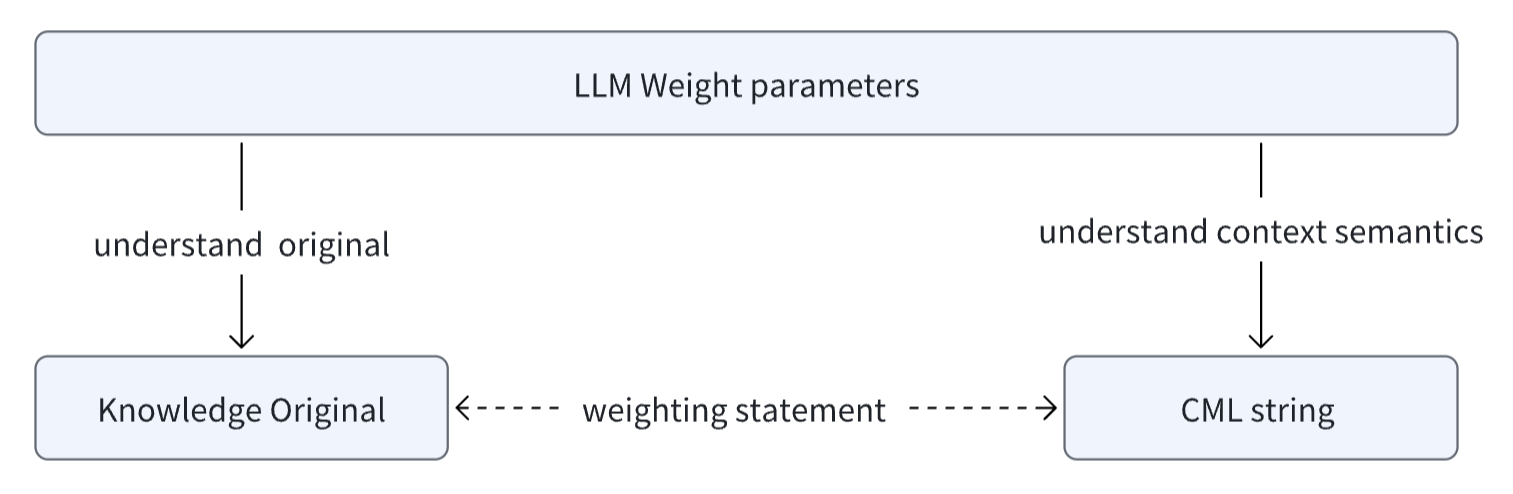
\includegraphics[width=0.8\linewidth]{assets/image-20250419104035008.png}
\end{figure}


From the perspective of knowledge governance architecture, the CSE
paradigm advocates a ``separation of powers'' among original knowledge
content, contextual annotations, and LLM weights, rather than distilling
all semantic and knowledge content entirely into the model's weight
parameters.

\subsubsection{3.7. Format Encoding}\label{37-format-encoding}

On top of freely composable semantic expressions, formalized encoding is
applied to produce the final contextual semantic markup.

\begin{itemize}
\item
  The plaintext format is designed for human readability, compatible
  with Markdown syntax, and easy to write.
\item
  At the same time, an encoded format is supported to eliminate
  delimiter ambiguity and special character issues, effectively avoiding
  the hassle of escaping and format corruption {[}13{]}. Since strings
  are the primitive value type across all mainstream data formats, CSE
  expressions can seamlessly integrate with existing frameworks,
  formats, and syntaxes. With simple encoding, they can be safely used
  in any embedding, nesting, storage, or transmission
  scenario---including but not limited to JSON, YAML, HTML, SQL, URLs,
  regular expressions, and shell commands.
\end{itemize}

\begin{figure}[htbp]
\centering
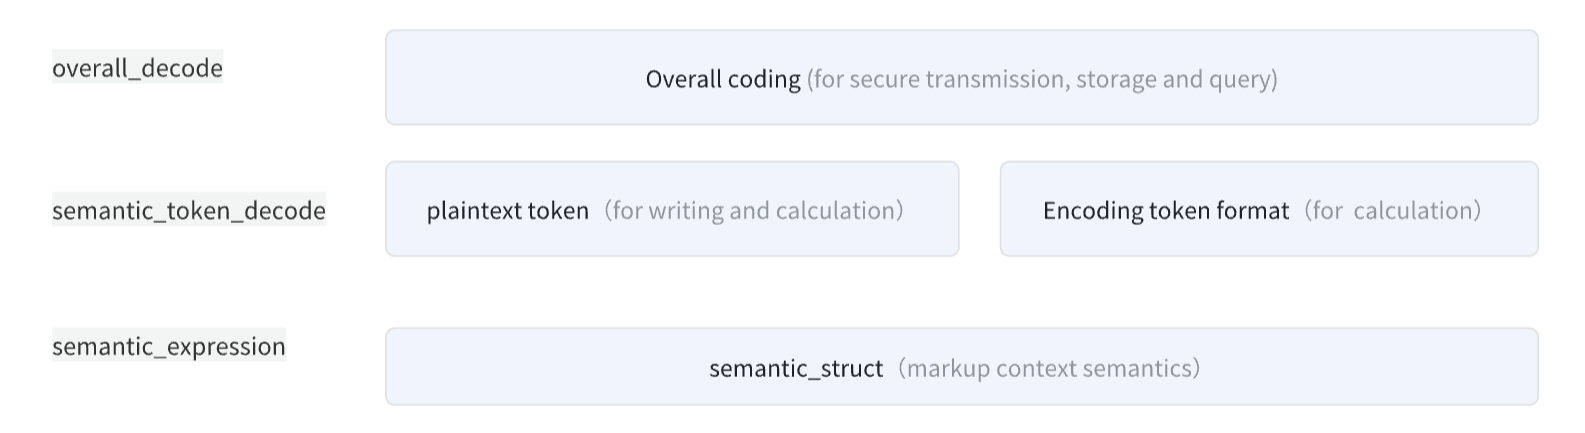
\includegraphics[width=0.8\linewidth]{assets/image-20250418111424824.png}
\end{figure}


\subsubsection{3.8. Semantic Structure}\label{38-semantic-structure}

Relation separators (\texttt{\textless{}separator\textgreater{}}) are
responsible not only for connecting semantic tokens in the expression
form, but also for carrying the semantic meaning of the structure
itself.

The design of relation separators is one of the core challenges in the
CSE paradigm. It involves a minimal completeness conjecture centered on
"relation-first semantic expression" {[}14{]} --- specifically, what
primitive structures to adopt, what types of relational semantics to
represent, and how to assign precedence among them.

This area intentionally leaves design space open for markup languages,
and CML is not necessarily the optimal solution.

\subsection{4. CML Language
Specification}\label{4-cml-language-specification}

CML (Context Mark Language), as the concrete implementation of the CSE
paradigm, builds upon the semantic architecture and expression forms
described above. It further specifies the scope of semantic structures,
precedence rules, symbol representation, and encoding rules for semantic
strings.

\subsubsection{4.1. Symbol
Representation}\label{41-symbol-representation}

In terms of form, CML selects five single-byte symbols that closely
align with natural semantics---:, ., @, +, and (space)---to serve as
relational separators. It also defines structural semantics and explicit
precedence levels for each.

\subsubsection{4.2. Semantic Structures}\label{42-semantic-structures}

The five relation separators in CML are semantic structural primitives
abstracted around three core requirements: priority expression of
tokens, structural extensibility, and logical orthogonality. These
primitives possess a high degree of expressiveness and combinability,
serving as the fundamental building blocks for constructing all forms of
logical-semantic relationships.

These five structural primitives are categorized into three types:
\texttt{basic\ structures}, \texttt{composite\ structures}, and
\texttt{compound\ structures}.

\begin{itemize}
\item
  Basic structures define simple structural relationships among multiple
  semantic tokens and can also serve as components within composite
  structures.
\item
  Composite structures are built from multiple basic structures.
\item
  Compound structures, on the other hand, are more macro-level container
  types that can link together any combination of semantic tokens, basic
  structures, and composite structures.
\end{itemize}

\paragraph{4.2.1. Supplementary
Relations}\label{421-supplementary-relations}

This is a basic structure. The semantic object on the right serves as a
supplementary explanation, specification, or constraint to the semantic
object on the left. Typically, it adds semantic detail without altering
the original semantic structure.

\[ f : A \ni B \ni C \]

This relationship is represented by the symbol \texttt{@}. The further
to the left a token appears, the higher its implicit
priority---indicating it should carry more semantic weight.

For example:

\begin{itemize}
\item
  \texttt{name}@\texttt{identity}@\texttt{organization}
\item
  \texttt{name}@\texttt{company}@\texttt{position}
\end{itemize}

The priority weight declarations for these two sets of tags are
different, but the focus of both is to emphasize
\textquotesingle name\textquotesingle{} first

\paragraph{4.2.2. Linear Progression
Relations}\label{422-linear-progression-relations}

This is a basic structure representing an ordered, step-by-step semantic
relationship. It can describe a wide range of directional flows such as:
progression, transformation chains, causal chains, sequences,
refinements, and lifecycle stages.

\[f: A \rightarrow B \rightarrow C\]

The symbol \texttt{.} is used to express this relation. Whether the
left-hand side carries slightly more semantic weight than the right is
context-dependent; the LLM is expected to infer the relative priority
based on the actual semantic tokens involved.

Examples:

\begin{itemize}
\item
  \texttt{biological}.\texttt{animal}.\texttt{human} --- the emphasis is
  on \texttt{human} as a subclass in this progression.
\item
  \texttt{product\_design}.\texttt{development}.\texttt{operations} ---
  based on the tokens themselves, it clearly describes a semantic
  lifecycle.
\end{itemize}

\paragraph{4.2.3. Parallel Set
Relations}\label{423-parallel-set-relations}

This is a basic structure where multiple semantic elements are presented
in parallel---akin to a set, a group of object attributes, or a
multi-branch description---with no implied priority or sequence. The
elements can be rearranged without altering the meaning.

\[f:\{A, B, C\}\]

The symbol \texttt{+} is used to represent this structure, indicating
equal weight among the tokens.

Examples:

\begin{itemize}
\item
  \texttt{man} + \texttt{woman} --- relative to the concept of , the
  combination order doesn\textquotesingle t matter.\texttt{human}
\item
  \texttt{name} + \texttt{age} + \texttt{username} --- all are part of a
  user's registration information.
\end{itemize}

\paragraph{4.2.4. Mapping Relations}\label{424-mapping-relations}

This is a compound correspondence between one semantic structure and
another, in a key-value (k-v) format. Both sides can use the basic
relationships described above, supporting two-dimensional semantic
expression.

\[ f(A, B) \mapsto f(C, D, E) \]

The \texttt{:} symbol is used to represent this structure. It is similar
to a key-value pair but offers more flexibility in construction. Both
the key and value parts can use basic structures, not just primitive
semantic tokens.

\begin{lstlisting}[
    basicstyle=\footnotesize\ttfamily,
    breaklines=true,
    breakatwhitespace=true,
    postbreak=\mbox{\textcolor{red}{$\hookrightarrow$}\space},
    columns=flexible,
    keepspaces=true,
    showstringspaces=false,
    frame=single,
    xleftmargin=2pt,
    xrightmargin=2pt,
    aboveskip=5pt,
    belowskip=5pt,
    literate={<}{{$\langle$}}1 {>}{{$\rangle$}}1
]
<key-context-struct>:<value-context-struct>
\end{lstlisting}

Examples of valid mapping semantic structures:

\begin{itemize}
\item
  \texttt{website}: \texttt{doc-war.com}
\item
  \begin{sloppypar}
  \texttt{website}@\texttt{doc-war.com}:
  \texttt{Document\ Battlefield}@\texttt{Contribution\ Judgement\ Value}
  \end{sloppypar}
\item
  \texttt{AI}+\texttt{LLM}:
  \texttt{ChatGPT}+\texttt{Claude}@\texttt{v3.7}
\item
  \begin{sloppypar}
  \texttt{ask}.\texttt{answer}:
  \texttt{Please\ introduce\ CML\ language?}.\texttt{CML\ language\ is\ a\ semantic\ structure\ language\ that\ aligns\ with\ natural\ semantics}
  \end{sloppypar}
\end{itemize}

\paragraph{Special Constraints}\label{special-constraints}

CML does not support nested mappings, in order to avoid increasing the
parsing complexity of the semantic structure itself. For example,
expressions like \texttt{user:ZhangSan:delete+query} are considered
invalid in format.

\paragraph{4.2.5. Combination Relation}\label{425-combination-relation}

Multiple semantic structures combine to form a new semantic whole,
without losing their original meaning. Conversely, splitting them also
preserves the meaning. Essentially, this is a computable "relation
structure container."

\[f(A)+f(B) =f(A+B)
\\
f(A) =f(A+B) - f(B)\]

The \texttt{space} symbol represents the semantic overlay of any two
structures.

"Because the space symbol has the lowest semantic priority, and the
order of the two sides (left or right) does not affect priority, it also
serves as the overall operator for CML strings. By using a space to
naturally concatenate two plaintext CML strings into a new CML string,
the result is still a valid CML string that does not alter the original
semantic meaning."

\[plaintext(A)+space+plaintext(B) = plaintext(A+space+B)\]

This lossless restoration characteristic of freely splitting and
rejoining CML strings endows them with semantic operability, not merely
serving as a semantic expression. It provides a solid foundation for
collaborative work in tagging.

\paragraph{Special Constraints}\label{special-constraints-details}

Since \texttt{space} serves the role of a lossless semantic operation,
expressions like \texttt{if\ user:ZhangSan\ is\ how} are technically
valid in format but will break the principle of lossless combination.
When multiple semantic strings are split and recombined, their meaning
will be disrupted due to the change in position.

\subsubsection{4.3. Operation Priority}\label{43-operation-priority}

Relational operations in CML are similar to the expression parsing in
programming languages: lexical scanning is performed from left to right,
and then, based on the priority of the relational separators, the order
of semantic operations is determined.

CML defines explicit priorities to ensure consistency in semantic
interpretation during tagging and inference stages:

\begin{lstlisting}[
      basicstyle=\scriptsize\ttfamily,
      breaklines=true,
      breakatwhitespace=false,
      breakindent=0pt,
      postbreak=\mbox{\textcolor{red}{$\hookrightarrow$}\space},
      columns=flexible,
      keepspaces=true,
      showstringspaces=false,
      frame=none,
      xleftmargin=20pt,
      xrightmargin=2pt
  ]
Supplementary>LinearProgressive>ParallelSet>Mapping>Combination
  \end{lstlisting}

\subsubsection{4.4. Minimal Completeness}\label{44-minimal-completeness}

The five relationship separators are abstracted from the semantic
structures of natural language and are the result of deep consideration
regarding ambiguity in expression and the controllability of structure.

\paragraph{4.4.1. Natural Language
Reference}\label{441-natural-language-reference}

The five relational separators defined in CML are inspired by the most
fundamental semantic structures implicitly found in natural language:
modification, sequential progression, parallel listing,
contrast/mapping, and combination.

\begin{lstlisting}[
    basicstyle=\footnotesize\ttfamily,
    breaklines=true,
    breakatwhitespace=true,
    postbreak=\mbox{\textcolor{red}{$\hookrightarrow$}\space},
    columns=flexible,
    keepspaces=true,
    showstringspaces=false,
    frame=single,
    xleftmargin=2pt,
    xrightmargin=2pt,
    aboveskip=5pt,
    belowskip=5pt
]
Examples from natural language:
Example: "The `man`A `tall`B `wearing a hat`C"       (A<-B<-C)
Example: "He `woke up`A, `got dressed`B, and `went out`C"            (A->B->C)
Example: "I like `apples`A, `bananas`B, and `oranges`C."       \{A, B, C\}
Example: "`ChatGPT`A, `Claude`B, and `DeepSeek`C are all `AI`D, also known as `LLM`E"        (A+B+C -> D+E)
Example: "`This flower`A + `is beautiful`B = `This flower is beautiful`A+B                              (A+B=AB)
\end{lstlisting}


Theoretically, by combining these five relational primitives, one can
express the vast majority of logical relationships. This gives the
system a high degree of completeness.

\paragraph{4.4.2. Semantic Within
Tokens}\label{442-semantic-within-tokens}

For logical relations like exclusion, quantifier ranges, or nested
mappings, CML does not support them natively at the structural level.
Instead, it delegates them to the token level, to be used in conjunction
with supplementary relationships, avoiding structural pollution and
reducing complexity in both precedence operations and human readability.

Because tokens themselves can also express structure.

\begin{lstlisting}[
    basicstyle=\footnotesize\ttfamily,
    breaklines=true,
    breakatwhitespace=true,
    postbreak=\mbox{\textcolor{red}{$\hookrightarrow$}\space},
    columns=flexible,
    keepspaces=true,
    showstringspaces=false,
    frame=single,
    xleftmargin=2pt,
    xrightmargin=2pt,
    aboveskip=5pt,
    belowskip=5pt
]
Natural language example:
  "Age about 18 to 25, and definitely not Chinese."
  (The token itself can imply range or exclusion structures)
Annotation:
  [X] `age`:`range`:`18-25`        (Invalid nesting, completely unnecessary---can be merged earlier or later)
  [X] `age`:`>18`+`<25`            (Overly fine-grained and unnecessary splitting)
  [ok] `age`:`range:18-25`          (Nesting within the token aligns with natural semantics)
  [ok] `age`:`18-25`
\end{lstlisting}



This reflects the \textbf{principle of structural minimalism}:

The CSE paradigm does not attempt to explicitly resolve all structural
semantic ambiguities in advance. Instead, it leverages the semantic
tokens connected by relational separators as the context for
interpreting relationships, enabling the LLM to infer the most
reasonable semantic relationships and corresponding weight priorities.

\paragraph{4.4.3. The Core Value of Explicit
Structure}\label{443-the-core-value-of-explicit-structure}

Skillfully expressing semantic structure within tokens also highlights
CML's core value in explicit encoding.

CML approximates---but is not equal to---natural language. Beyond
expressing weighted core semantics, it serves a critical expressive
purpose. Unlike natural language reasoning, where token segmentation is
uncontrollable, explicit segmentation in CML allows for vertical
layering and horizontal relationship delineation in semantics. This
eliminates relational ambiguity and ultimately enhances controllability
and interpretability.

\subsubsection{4.5. Encoding Rules}\label{45-encoding-rules}

Based on semantic expression, CML defines two standard string formats.
The core difference lies in which object, at what stage, and in what
form, wraps the semantic token (\texttt{semantic\_token}).

\begin{figure}[htbp]
\centering
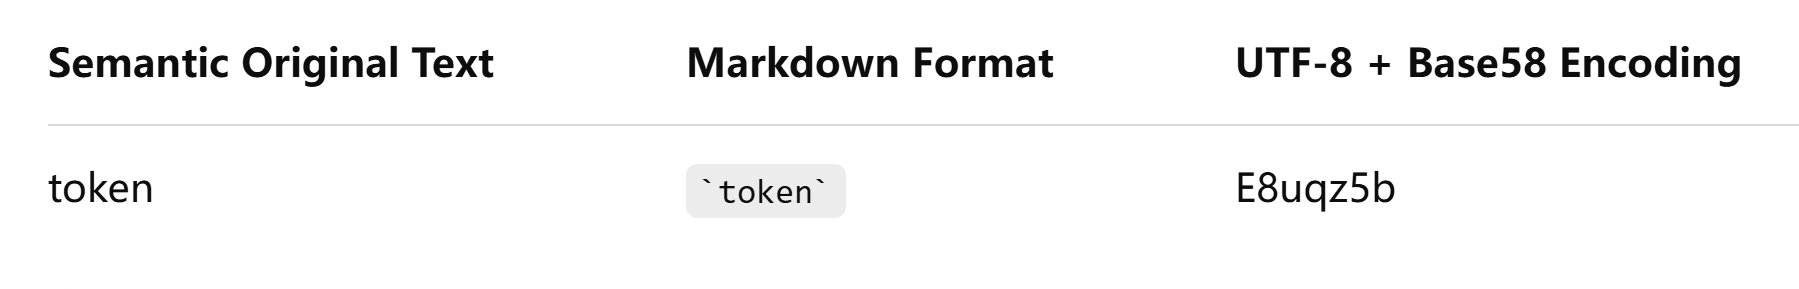
\includegraphics[width=0.8\linewidth]{assets/image-20250421172756701.png}
\end{figure}

\paragraph{4.5.1. Natural Language
Format}\label{451-natural-language-format}

The natural language format is designed for documentation engineers to
write in plain text, suitable for human-readable scenarios.

It uses Markdown syntax (specifically, \emph{inline code} with
backticks) {[}15{]} to wrap semantic tokens (\texttt{semantic\_token}).
Documentation engineers can work within a WYSIWYG Markdown editor,
making it fast and intuitive to edit semantic structures in plain text.

For example, writing the following plain-text string in Markdown:

\begin{lstlisting}[
    basicstyle=\footnotesize\ttfamily,
    breaklines=true,
    breakatwhitespace=true,
    postbreak=\mbox{\textcolor{red}{$\hookrightarrow$}\space},
    columns=flexible,
    keepspaces=true,
    showstringspaces=false,
    frame=single,
    xleftmargin=2pt,
    xrightmargin=2pt,
    aboveskip=5pt,
    belowskip=5pt
]
`token1`.`token2`@`token3`+`token4` `token5`:`token6`
\end{lstlisting}

Will instantly render into the following clear and readable semantic
structure:\texttt{token1}.\texttt{token2}@\texttt{token3}+\texttt{token4}
\texttt{token5}:\texttt{token6}

\paragraph{4.5.2. Encoded Format}\label{452-encoded-format}

CML strings that include backticks (`)---including the separators---may,
in certain special scenarios, lead to unexpected parsing boundaries or
escaping issues.

To address this, and to support use cases such as embedding, storage,
parsing, and computation, CML defines a more secure and consistent
encoded output format.

\begin{figure}[htbp]
\centering
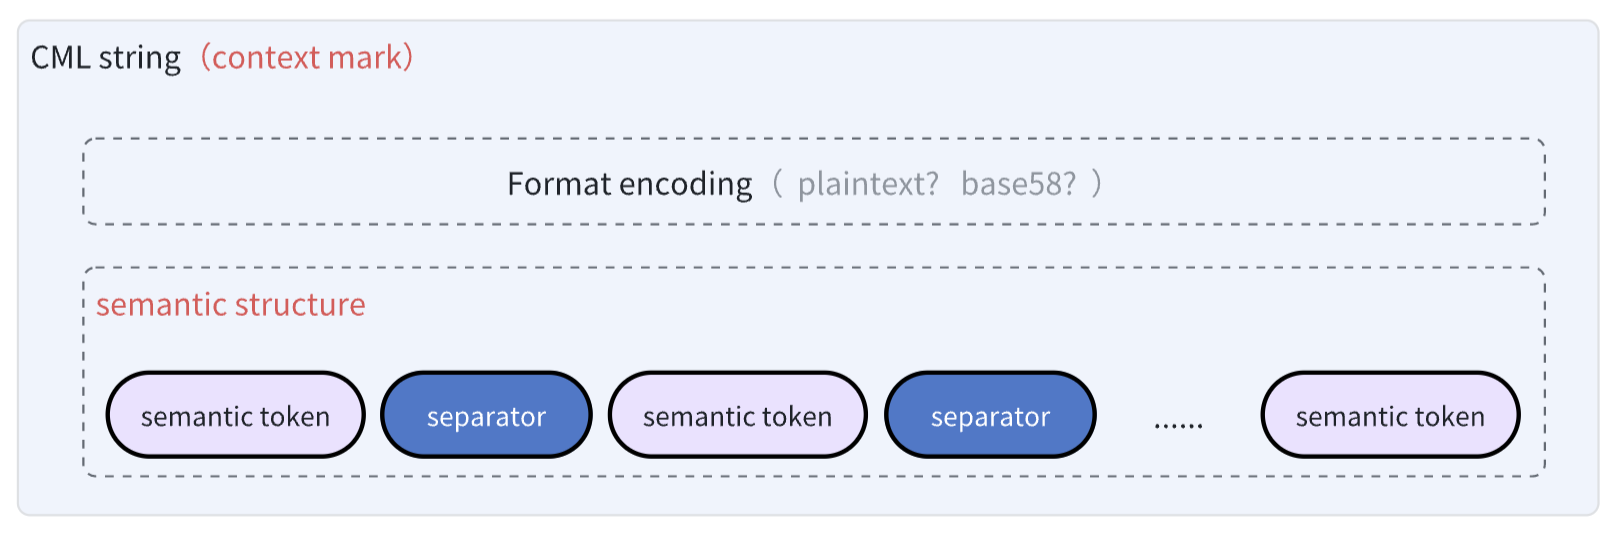
\includegraphics[width=0.8\linewidth]{assets/image-20250418171524138.png}
\end{figure}

Example

\begin{lstlisting}[
    basicstyle=\footnotesize\ttfamily,
    breaklines=true,
    breakatwhitespace=true,
    postbreak=\mbox{\textcolor{red}{$\hookrightarrow$}\space},
    columns=flexible,
    keepspaces=true,
    showstringspaces=false,
    frame=single,
    xleftmargin=2pt,
    xrightmargin=2pt,
    aboveskip=5pt,
    belowskip=5pt
]
`token1`.`token2`@`token3`+`token4` `token5`:`token6`
\end{lstlisting}

To encode the above plain-text CML string into its encoded format,
follow these steps:

\begin{enumerate}
\def\labelenumi{\arabic{enumi}.}
\item
  Extract semantic tokens and separators From the original CML string,
  extract all \texttt{semantic\ tokens} (text within backticks) and
  \texttt{relationship\ separators} (e.g., \texttt{.}, \texttt{@},
  \texttt{+}, \texttt{}, \texttt{:}).
\item
  For each semantic token, its original text (excluding the backticks)
  is first encoded into a byte stream using UTF-8, and then this byte
  stream is Base58 encoded {[}16{]} to generate a Base58 string.
\end{enumerate}

\begin{lstlisting}[
    basicstyle=\footnotesize\ttfamily,
    breaklines=true,
    breakatwhitespace=true,
    postbreak=\mbox{\textcolor{red}{$\hookrightarrow$}\space},
    columns=flexible,
    keepspaces=true,
    showstringspaces=false,
    frame=single,
    xleftmargin=2pt,
    xrightmargin=2pt,
    aboveskip=5pt,
    belowskip=5pt
]
token1 -> encoded -> zyvFCwFv
token2 -> encoded -> zyvFCwFw
token3 -> encoded -> zyvFCwFx
token4 -> encoded -> zyvFCwFy
token5 -> encoded -> zyvFCwFz
token6 -> encoded -> zyvFCwG1
\end{lstlisting}


\begin{enumerate}
\def\labelenumi{\arabic{enumi}.}
\item
  Next, replace the encoded tokens back into the original string; in
  other words, Base58 encoding takes over the wrapping function of
  backticks.
\end{enumerate}

\begin{lstlisting}[
    basicstyle=\footnotesize\ttfamily,
    breaklines=true,
    breakatwhitespace=true,
    postbreak=\mbox{\textcolor{red}{$\hookrightarrow$}\space},
    columns=flexible,
    keepspaces=true,
    showstringspaces=false,
    frame=single,
    xleftmargin=2pt,
    xrightmargin=2pt,
    aboveskip=5pt,
    belowskip=5pt
]
zyvFCwFv.zyvFCwFw@zyvFCwFx+zyvFCwFy zyvFCwFz:zyvFCwG1
\end{lstlisting}

\begin{enumerate}
\def\labelenumi{\arabic{enumi}.}
\item
  Finally, the entire result is encoded again using UTF-8+Base58,
  eliminating all special characters.
\end{enumerate}

\begin{lstlisting}[
    basicstyle=\footnotesize\ttfamily,
    breaklines=true,
    breakatwhitespace=true,
    postbreak=\mbox{\textcolor{red}{$\hookrightarrow$}\space},
    columns=flexible,
    keepspaces=true,
    showstringspaces=false,
    frame=single,
    xleftmargin=2pt,
    xrightmargin=2pt,
    aboveskip=5pt,
    belowskip=5pt
]
3EkzyE8r5SqnU6KSbLS98LVLJxFoNvskzaazkuEEryWminqaGwJz13YoatvfoRWoDyrofwUCQ
\end{lstlisting}

\paragraph{4.5.3. Line Breaks and Multi-space
Compatibility}\label{453-line-breaks-and-multi-space-compatibility}

In natural text editing scenarios, especially when handling longer
contexts, users often insert line breaks (\textbackslash n,
\textbackslash r\textbackslash n, \textbackslash r) to improve
readability or add consecutive multiple spaces for visual separation,
which is a natural practice.

Therefore, CML editors should support preprocessing robustness by
uniformly converting all types of line breaks and excessive spaces into
a single space before performing Base58 encoding.

\subsection{5. Comparison Between CML and Other
Approaches}\label{5-comparison-between-cml-and-other-approaches}

Currently, there are no systematic solutions identified in this field
that address this issue. As of the date of this paper's publication, no
literature has been found that proposes a paradigm based on dynamic
semantic expression, nor any papers related to Context Markup Language
(CML), or Large Language Model (LLM) governance architectures designed
from the perspective of the semantic lifecycle, including relevant tools
or documentation.

The industry is still dominated by static structural languages such as
JSON, YAML, and RDF, or their improved versions, which are used to
support semantic expression, storage, and exchange.

\subsubsection{5.1. JSON-LD vs CML}\label{51-json-ld-vs-cml}

Among them, JSON-LD, which is compatible with JSON, is currently
considered one of the most advanced static semantic expression formats,
especially in the areas of web semantics and structured data annotation.

On one hand, it utilizes the schema.org standardized vocabulary {[}17{]}
for semantic expression, which is a semantic annotation approach
supported by major search engines. On the other hand, by
using\texttt{\textless{}script\ type="application/ld+json"\textgreater{}}
, it allows for embedding a snippet of "machine-readable" structured
data into an HTML page. This data is not rendered by the browser and
does not affect the visual appearance or layout of the webpage, thus
offering a non-intrusive way of semantic expression.

Here is a typical example in JSON-LD format:

\begin{lstlisting}[
    basicstyle=\footnotesize\ttfamily,
    breaklines=true,
    breakatwhitespace=true,
    postbreak=\mbox{\textcolor{red}{$\hookrightarrow$}\space},
    columns=flexible,
    keepspaces=true,
    showstringspaces=false,
    frame=single,
    xleftmargin=2pt,
    xrightmargin=2pt,
    aboveskip=5pt,
    belowskip=5pt,
]
{
  "@context": "https://schema.org",
  "@type": "Article",
  "headline": "A New Paradigm: Redefining Knowledge Discovery",
  "author": {
    "@type": "Person",
    "name": "lilei"
  }
}
\end{lstlisting}

However, it is important to note that schema.org enumerates over 2,000
terms. Such an extensive static semantic specification imposes excessive
demands on manual annotation, which can negatively impact annotation
quality. Even professional engineers may find it difficult to quickly
master every term and its semantic nuance. In the era of LLMs, this
approach appears to be "too heavy".

This is precisely why CML defines only five relation delimiters in a
minimalist way --- I hope for CML to become the Markdown of semantic
annotation, rather than another HTML.

\subsubsection{5.2. JSON Lines vs. CML
String}\label{52-json-lines-vs-cml-string}

Moreover, the nested structure of JSON-LD is highly complex and
inefficient to parse in large-scale annotation scenarios, making it less
suitable for mainstream use in the LLM field. In contrast, LLMs tend to
prefer an alternative approach---JSON Lines {[}18{]}---which enables
incremental writing/streaming processing (line by line).

JSON Lines is widely used by platforms such as OpenAI, Hugging Face, and
FastChat for fine-tuning and training data formats.

This format separates each single-line JSON object with a newline
character (\texttt{\textbackslash{}n} ), allowing each line to be read
and parsed independently without loading the entire file at once.

Here is an example of a file:\texttt{example.jsonl}

\begin{lstlisting}[
    basicstyle=\footnotesize\ttfamily,
    breaklines=true,
    breakatwhitespace=true,
    postbreak=\mbox{\textcolor{red}{$\hookrightarrow$}\space},
    columns=flexible,
    keepspaces=true,
    showstringspaces=false,
    frame=single,
    xleftmargin=2pt,
    xrightmargin=2pt,
    aboveskip=5pt,
    belowskip=5pt,
]
{"id": 1, "prompt": "Hello", "response": "Hello, how can I help you?"}
{"id": 2, "prompt": "What is JSONL?", "response": "JSON Lines is a structured text format."}
{"id": 3, "prompt": "Thank you", "response": "You're welcome!"}
\end{lstlisting}


Compared to JSON, the key innovation of JSON Lines lies in its use of as
a relationship delimiter for composition. This concept is remarkably
similar to CML's use of space(\texttt{}) as a composition operator.
CML strings obviously also support incremental writing/streaming.

However, JSON Lines requires file-based storage and is not ideal for use
as an embedded data format. Additionally, since each line must be parsed
as a full JSON object, the segmentation process incurs a higher
computational overhead---especially when dealing with large volumes of
data. In contrast, CML\textquotesingle s use of single-string slicing is
significantly more efficient in such contexts.`

\subsection{6. Conclusion and Future
Work}\label{6-conclusion-and-future-work}

The CSE paradigm and the design of CML represent not only a structural
innovation in single-string semantic expression, but also a conceptual
shift in semantic methodology---offering a fresh perspective on the
architectural design of next-generation LLMs and their semantic
lifecycle.

Looking ahead, both CSE and CML hold significant value for theoretical
research and engineering practice. They have the potential to become
foundational elements of semantic infrastructure in the AI era, serving
as a structured semantic intermediate language across the ecosystem. As
the capabilities of large models continue to grow, semantic expression,
organization, and reasoning are likely to emerge as core
competencies---and key differentiators---of next-generation LLMs.

This paper encourages the industry to pay close attention to the
theoretical framework and transformative potential of this paradigm, and
calls for more visionary contributors to join the effort of promoting
CSE and CML as a globally accepted standard for semantic expression and
collaboration.

As the author's first systematic research paper in the open-source
domain, this work strives for rigor and structure. However, as an
independent researcher, limitations in resources, influence, and
interdisciplinary collaboration inevitably lead to areas of
imperfection. This paper is a humble starting point, intended to spark
broader academic discussion and practical exploration. It is my hope to
further refine this semantic paradigm in collaboration with more
research teams and industry organizations, and to contribute to the
advancement of structured semantics in real-world applications.

Open-source project repository: \url{https://github.com/ContextMark/CML}

\subsection{References}\label{references}

{[}1{]} B. Thompson, ``AI will drive the cost of intelligence to zero?
Not so fast,'' \emph{Medium}, Nov. 10, 2024. {[}Online{]}. Available:
\url{https://medium.com/the-generator/ai-will-drive-the-cost-of-intelligence-to-zero-not-so-fast-d90d901baf10}.
{[}Accessed: Apr. 2025{]}.

{[}2{]} S. Pandey, "Retrieval-Augmented Generation (RAG): Improving
AI\textquotesingle s Answer with External Knowledge," \emph{Medium},
Oct. 24, 2024. {[}Online{]}. Available:
\url{https://medium.com/@santoshpandey987/retrieval-augmented-generation-rag-improving-ais-answer-with-external-knowledge-7961641e9fde}.
{[}Accessed: Apr. 2025{]}.

{[}3{]} K. Cagle, "JSON-LD rewrites the Semantic Web," \emph{LinkedIn},
Sep. 13, 2017. {[}Online{]}. Available:
\url{https://www.linkedin.com/pulse/json-ld-rewrites-semantic-web-kurt-cagle}.
{[}Accessed: Apr. 2025{]}.

{[}4{]} C. Qian, S. Xing, S. Li, Y. Zhao, and Z. Tu, ``DecAlign:
Hierarchical Cross-Modal Alignment for Decoupled Multimodal
Representation Learning,'' \emph{arXiv}, Mar. 14, 2025. {[}Online{]}.
Available: \url{https://arxiv.org/abs/2503.11892}. {[}Accessed: Apr. 20,
2025{]}.

{[}5{]} Wikipedia contributors, ``DOGMA,'' \emph{Wikipedia, The Free
Encyclopedia}, Apr. 20, 2025. {[}Online{]}. Available:
\url{https://en.wikipedia.org/wiki/DOGMA}. {[}Accessed: Apr. 20,
2025{]}.

{[}6{]} S. Pimparkhede et al., ``DocCGen: Document-based Controlled Code
Generation,'' \emph{arXiv}, Jun. 2024. {[}Online{]}. Available:
\url{https://arxiv.org/abs/2406.11925}. {[}Accessed: Apr. 20, 2025{]}.

{[}7{]} N. P. Ding et al., ``Knowledge Prompt Chaining for Semantic
Modeling,'' \emph{arXiv}, Jan. 2025. {[}Online{]}. Available:
\url{https://arxiv.org/abs/2501.08540}. {[}Accessed: Apr. 20, 2025{]}.

{[}8{]} X. Tan et al., ``Struct-X: Enhancing Large Language Models
Reasoning with Structured Data,'' \emph{arXiv}, Jul. 2024. {[}Online{]}.
Available: \url{https://arxiv.org/abs/2407.12522}. {[}Accessed: Apr. 20,
2025{]}.

{[}9{]} Y. Liu et al., ``Generative AI-driven Semantic Communication
Networks,'' \emph{arXiv}, Jan. 2024. {[}Online{]}. Available:
\url{https://arxiv.org/abs/2401.00124}. {[}Accessed: Apr. 20, 2025{]}.

{[}10{]} ``Open Neural Network Exchange (ONNX),'' \emph{ONNX.ai},
{[}Online{]}. Available: \url{https://onnx.ai}. {[}Accessed: Apr. 20,
2025{]}.

{[}11{]} Anthropic, ``Interpretability Dreams,'' \emph{Anthropic}, May
24, 2023. {[}Online{]}. Available:
\url{https://www.anthropic.com/research/interpretability-dreams}.
{[}Accessed: Apr. 20, 2025{]}.

{[}12{]} Z. Li, Y. Wang, and H. Chen, ``Dynamic Skill Adaptation for
Large Language Models,'' \emph{arXiv}, Dec. 2024. {[}Online{]}.
Available: \url{https://arxiv.org/abs/2412.19361}. {[}Accessed: Apr. 20,
2025{]}.

{[}13{]} ``Escape character,'' \emph{Wikipedia}, Apr. 2025.
{[}Online{]}. Available:
\url{https://en.wikipedia.org/wiki/Escape_character}. {[}Accessed: Apr.
20, 2025{]}.

{[}14{]} S. Jauhar, ``A Relation-Centric View of Semantic Representation
Learning,'' \emph{Ph.D. dissertation}, Carnegie Mellon University, 2017.
{[}Online{]}. Available:
\url{https://www.cs.cmu.edu/~sjauhar/thesis.pdf}. {[}Accessed: Apr. 20,
2025{]}.

{[}15{]} ``Markdown,'' \emph{Wikipedia}, Apr. 2024. {[}Online{]}.
Available: \url{https://zh.wikipedia.org/wiki/Markdown}. {[}Accessed:
Apr. 2025{]}.

{[}16{]} ``Base58,'' \emph{Wikipedia}, Jan. 2025. {[}Online{]}.
Available: \url{https://zh.wikipedia.org/wiki/Base58}. {[}Accessed: Apr.
2025{]}.

{[}17{]} ``Schema.org,'' \emph{Wikipedia}, Apr. 2025. {[}Online{]}.
Available: \url{https://en.wikipedia.org/wiki/Schema.org}. {[}Accessed:
Apr. 2025{]}.

{[}18{]} ``JSON Lines,'' \emph{Wikipedia}, Mar. 2025. {[}Online{]}.
Available: \url{https://en.wikipedia.org/wiki/JSON_streaming\#JSONL}.
{[}Accessed: Apr. 2025{]}.

{[}19{]} C. Singh, J. P. Inala, M. Galley, R. Caruana, and J. Gao,
``Rethinking Interpretability in the Era of Large Language Models,''
\emph{arXiv preprint}, Jan. 30, 2024. {[}Online{]}. Available:
\url{https://arxiv.org/abs/2402.01761}. {[}Accessed: Apr. 2025{]}.

In terms of semantic paradigm thinking, the most cutting-edge conceptual
framework may come from Niu Kai and colleagues from Beijing University
of Posts and Telecommunications, China, in 2022. Their work aims to
advance the way of thinking about communication systems from the
"syntactic layer" of the traditional Shannon paradigm to the "semantic
layer", shifting the focus from "data compression" to "semantic
compression". Based on this foundational logic, they further proposed a
corresponding mathematical theory.

{[}20{]} K. Niu and P. Zhang, ``A Mathematical Theory of Semantic
Communication: Overview,'' \emph{arXiv preprint}, Jan. 25, 2024.
{[}Online{]}. Available: \url{https://arxiv.org/abs/2401.14160}.
{[}Accessed: Apr. 2025{]}.

{[}21{]} K. Niu, J. Dai, S. Yao, S. Wang, Z. Si, X. Qin, and P. Zhang,
``Towards Semantic Communications: A Paradigm Shift,'' \emph{arXiv
preprint}, Mar. 13, 2022. {[}Online{]}. Available:
\url{https://arxiv.org/abs/2203.06692}. {[}Accessed: Apr. 2025{]}.

% In the field of meta-linguistic structural research related to natural
% language, Professor Cui Xiliang from Beijing Language and Culture
% University presented some cognitive models in his article published in
% Issue 5 of \emph{Language Teaching and Linguistic Studies} in 2002.
% However, these models focus on the logical dimension rather than the
% underlying structural dimension.

% {[}22{]} X. C. Cui, ``认知语言学: 研究范围和研究方法(Cognitive
% Linguistics: Scope and Methodology),'' \emph{语言教学与研究}, no. 5, pp.
% 1--7, 2002. {[}Online{]}. Available:
% \url{https://fls.blcu.edu.cn/attach/0/1410161054566649318.pdf}.
% {[}Accessed: Apr. 2025{]}.

\end{document}
